% --------------------------------------------------- %
%						Capa						  %
% --------------------------------------------------- %
% >>> Capa Personalizada
\renewcommand{\imprimircapa}{%
	\begin{capa}%
		\center
		{\ABNTEXchapterfont\bfseries\large\imprimirINSTITUICAO}
			\vspace*{1.5cm}
		\includegraphics*[width=0.25\textwidth]{brasao_ufes.jpg}
			\vspace*{1.5cm} \\
		{\ABNTEXchapterfont\bfseries\Large\MakeUppercase\imprimirautor}
				\vspace*{2.5cm} \\
		{\ABNTEXchapterfont\bfseries\Large\imprimirtitulo}
			\vfill
			\vspace*{0.5cm}
		{\large\MakeUppercase\imprimirlocal}
		\par
		{\large\MakeUppercase\imprimirdata}
			\vspace*{1cm}
	\end{capa}
}

\imprimircapa

% --------------------------------------------------- %
%					Folha de Rosto 					  %
% --------------------------------------------------- %
% >> O * indica que haverá a ficha bibliográfica

\renewcommand{\imprimirfolhaderosto}{

\begin{folhaderosto}
	\begin{center}
    	{\ABNTEXchapterfont\large\imprimirautor}
		    \vspace*{\fill}\vspace*{\fill}
    	\begin{center}
	    	\ABNTEXchapterfont\bfseries\Large\imprimirtitulo
	    \end{center}
    		\vspace*{\fill}
    		\hspace{.45\textwidth}
	    \begin{minipage}{.5\textwidth}
        	\imprimirpreambulo
	    \end{minipage}
    		\vspace*{\fill}
	    \end{center}  
        \begin{center}
        	% >> Se necessáiro, ajustar os \vspace
        	%\vspace*{0.5cm}
        {\large\imprimirlocal}
        \par
        {\large\imprimirdata}
       		%\vspace*{1cm}
      \end{center}
\end{folhaderosto}
}

\imprimirfolhaderosto

% --------------------------------------------------- %
%					Ficha Catalográfica 			  %
% --------------------------------------------------- %

% Isto é um exemplo de Ficha Catalográfica, ou ``Dados internacionais de
% catalogação-na-publicação''. Você pode utilizar este modelo como referência. 
% Porém, provavelmente a biblioteca da sua universidade lhe fornecerá um PDF
% com a ficha catalográfica definitiva após a defesa do trabalho. Quando estiver
% com o documento, salve-o como PDF no diretório do seu projeto e substitua todo
% o conteúdo de implementação deste arquivo pelo comando abaixo:
%
% \begin{fichacatalografica}
%     \includepdf{fig_ficha_catalografica.pdf}
% \end{fichacatalografica}

%\begin{fichacatalografica}
%	\sffamily
%	\vspace*{\fill}					% Posição vertical
%	\begin{center}					% Minipage Centralizado
%	\fbox{\begin{minipage}[c][8cm]{13.5cm}		% Largura
%	\small
%	\imprimirautor
%	%Sobrenome, Nome do autor
%	
%	\hspace{0.5cm} \imprimirtitulo  / \imprimirautor. --
%	\imprimirlocal, \imprimirdata-
%	
%	\hspace{0.5cm} \pageref{LastPage} p. : il. (algumas color.) ; 30 cm.\\
%	
%	\hspace{0.5cm} \imprimirorientadorRotulo~\imprimirorientador\\
%	
%	\hspace{0.5cm}
%	\parbox[t]{\textwidth}{\imprimirtipotrabalho~--~\imprimirinstituicao,
%	\imprimirdata.}\\
%	
%	\hspace{0.5cm}
%		1. Palavra-chave1.
%		2. Palavra-chave2.
%		2. Palavra-chave3.
%		I. Orientador.
%		II. Universidade xxx.
%		III. Faculdade de xxx.
%		IV. Título 			
%	\end{minipage}}
%	\end{center}
%\end{fichacatalografica}

% --------------------------------------------------- %
%					Folha de Aprovação			      %
% --------------------------------------------------- %
% >>> Após apresentação do trabalho, substitua todo o conteúdo 
% por uma imagem da página assinada pela banca com o comando abaixo:
\ifisFolhaAprovacao
%TCC finalizado
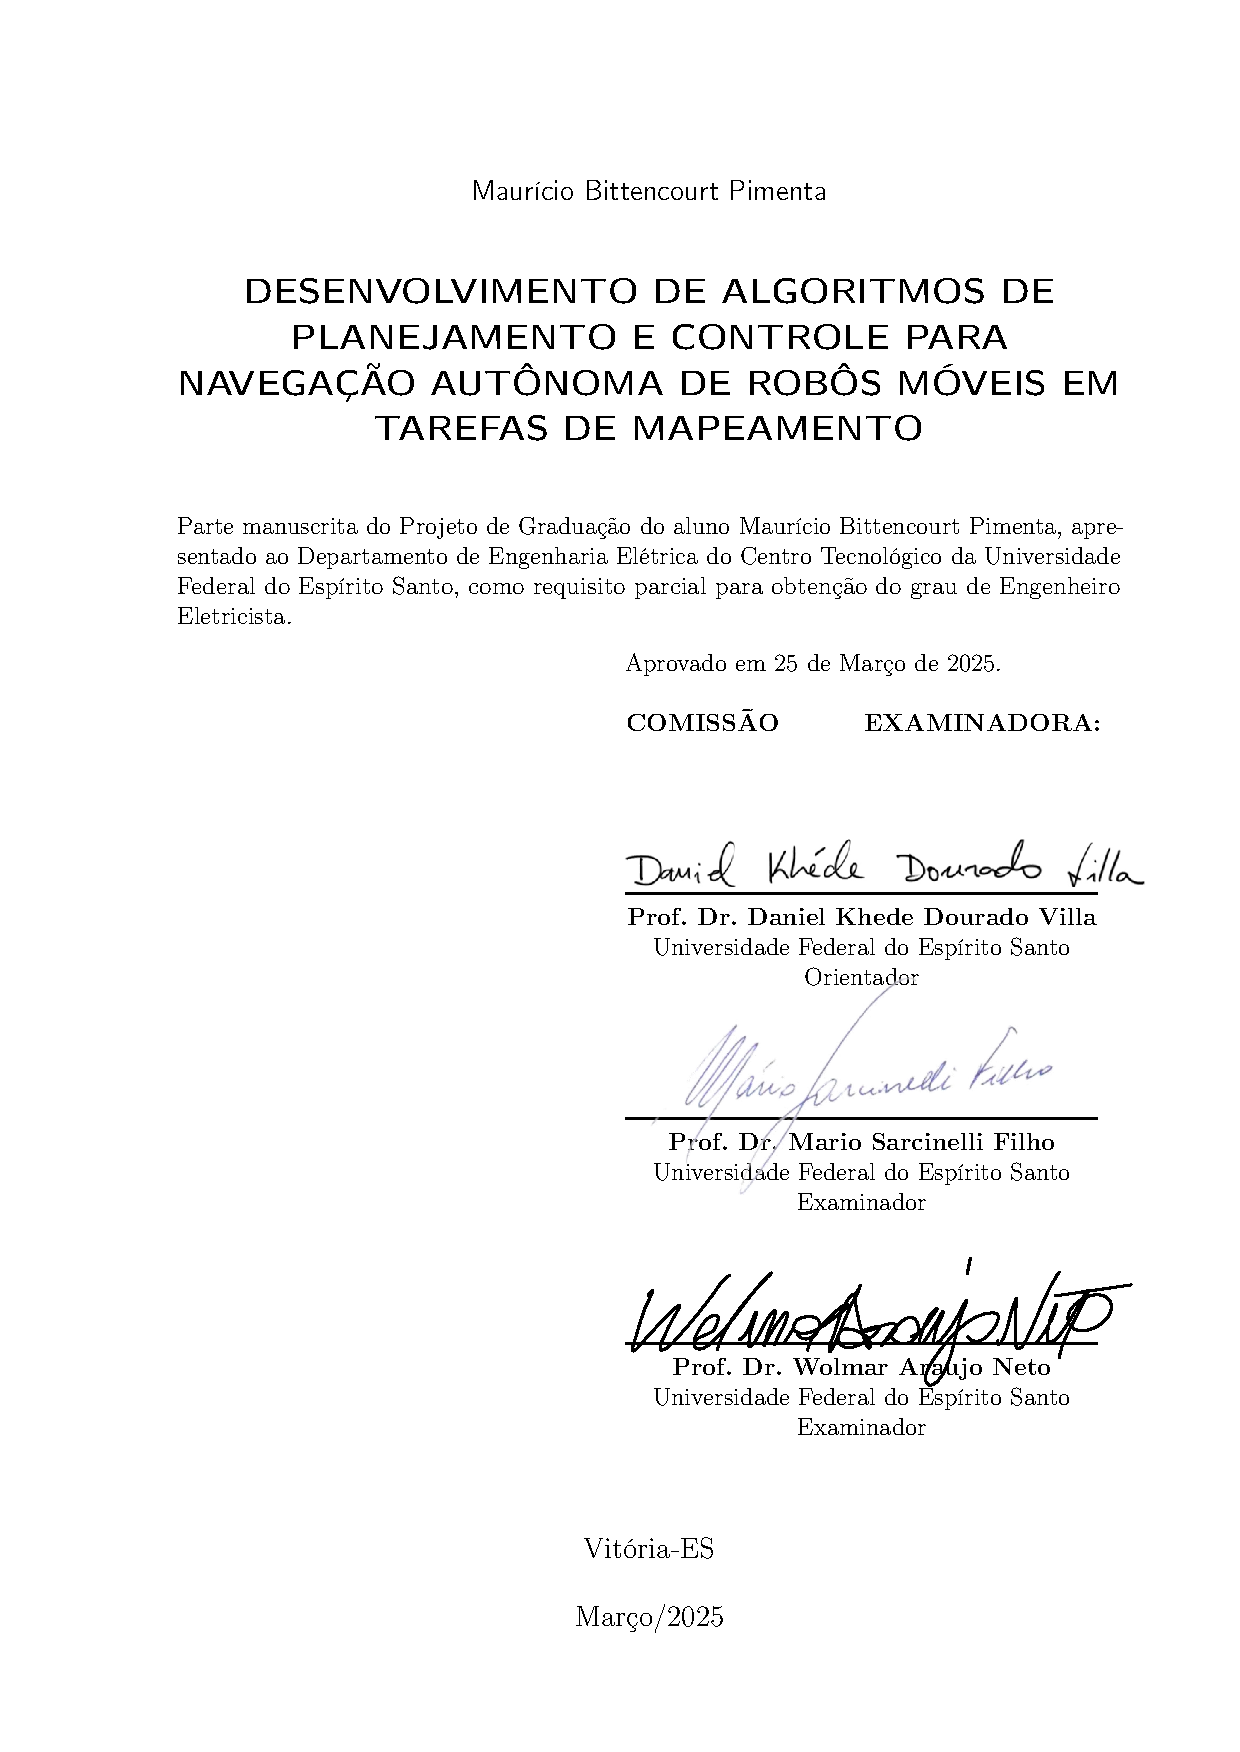
\includepdf{aprovacao.pdf}
\else
%TCC não finalizado
\begin{folhadeaprovacao}
   \begin{center}
     {\ABNTEXchapterfont\large\imprimirautor}
 	\begin{center}
      	\ABNTEXchapterfont\bfseries\Large\imprimirtitulo
     \end{center}
     %\vspace*{\fill}
   \end{center}    
     \imprimirpreambulo
 		\vspace{-0.5cm}
     \begin{center}
 		\hspace{.45\textwidth}
     \begin{minipage}{.5\textwidth}
         Aprovado em x de xxxx de 20xx. \\\\
         \textbf{COMISSÃO EXAMINADORA:}
         \vspace{0.5cm}
         \assinatura{\textbf{\imprimirorientador} \\ Universidade Federal do Espírito Santo \\ Orientador}
         %\vspace{1.0cm}
%        \assinatura{\textbf{\imprimircoorientador} \\ Universidade Federal do Espírito Santo \\ Coorientadora}
        \vspace{1.0cm}
 		\assinatura{\textbf{Prof. Dr. Mario Sarcinelli Filho} \\ Universidade Federal do Espírito Santo \\ Examinador}
 		\vspace{1.0cm}
 		\assinatura{\textbf{Prof. Dr. Wolmar Araujo Neto} \\ Universidade Federal do Espírito Santo \\ Examinador}
     \end{minipage}
 	    \vspace*{\fill}
    \end{center}
         
    \begin{center}
       	% >> Se necessáiro, ajustar os \vspace
 		%\vspace*{0.5cm}
     	{\large\imprimirlocal}
     	\par
     	{\large\imprimirdata}
    		%\vspace*{1cm}
   \end{center}  
 \end{folhadeaprovacao}
\fi
% --------------------------------------------------- %
%						Dedicatória				      %
% --------------------------------------------------- %
\begin{dedicatoria}
   \vspace*{\fill}
   \centering
   \noindent
   \textit{Dedicatória!!} \vspace*{\fill}
\end{dedicatoria}

% --------------------------------------------------- %
%					Agradecimentos				      %
% --------------------------------------------------- %

\begin{agradecimentos}

% Gostaria de agradecer a todas essas pessoas especiais que apareceram (e estão) na minha vida e que permitem que eu continue com os meus estudos. A todos vocês, minha eterna gratidão.

% Aos meus pais, Adan e Eva, pelo apoio e dedicação e xxxx.
    
% Ao minha/meu irmã@ Mari@ por todo apoio emocional e por me servir de inspiração.

% À minha/meu namorad@ Mari@ por toda compreensão e apoio durante toda a graduação.
    	
% A meu orientador Yann Lecun e coorientador Geoffrey Hinton por despertar meu interesse por esse tema fascinante e por toda ajuda, orientação e dedicação durante o desenvolvimento deste trabalho.

% Aos membros do Laboratório Visio, pelo xxxx.

% À banca examinadora pela aceitação do convite e pelo tempo investido para leitura e avaliação desse trabalho.

% Agradeço à Universidade Federal do Espirito Santo pela minha formação. 

% Finalmente, agradeço à Fundação de XXXX pelo apoio financeiro.
\end{agradecimentos}

% --------------------------------------------------- %
%						Epígrafe			      	  %	
% --------------------------------------------------- %

%\begin{epigrafe}
%    \vspace*{\fill}
%	\begin{flushright}
%		Insira a epígrafe aqui!
%	\end{flushright}
%\end{epigrafe}

% --------------------------------------------------- %
%						Resumo				      	  %	
% --------------------------------------------------- %

% Resumo em português
\setlength{\absparsep}{18pt} % ajusta o espaçamento dos parágrafos do resumo
\begin{resumo}

% \txr{\textbf{COMENTARIO GERAL:}} O resumo de um trabalho tem uma estrutura bem definida, explicada a seguir:
% \textbf{1. \txr{Contextualização}}
% Identifica qual é a grande área onde seu trabalho esta inserido e qual é a importância dessa grande área.
% \textbf{2. \txr{Gaps ou vazios}}
% Aqui o autor diz que coisa na grande área precisa ser pesquisada. 
% Aqui é onde o autor deixa claro o que ainda não esta bem entendido, esta em aberto ou é controvertido. 
% Em resumo, o Gap é o vazio dessa grande área na qual  o trabalho esta inserido. 
% O comum é iniciar con as palavras: \textit{ainda}, \textit{Sem embargo}
% \textbf{\txr{3. Proposta}}
% Em esta parte o autor indica qual é o proposta e o objetivo do trabalho, evidentemente o objetivo deve estar relacionado con el Gap. O comum é iniciar con as frases: \textit{Este trabalho descreve ...}; \textit{Este trabalho reporta ...}; \textit{Aqui, ...}; \textit{Em este trabalho, é proposto, ... }.
% \textbf{\txr{4. Metodologia}}
% Aqui são descritos os métodos utilizados para a realização do trabalho.
% \textbf{\txr{5. Resultados}}
% Esta parte do resumo é extremadamente importante, não existe resumo que não tenha seção de resultados bem clara e detalhada, cabe ao autor identificar qual é seu principal resultado, para deixar bem claro no resumo.  Acontinuação um exemplo.

% \textbf{1. \txr{Contextualização}}
% O câncer de pele é o tipo de câncer mais comum no Brasil. 
% O melanoma é seu subtipo mais mortal. 
% Portanto, é essencial que seja detectado em seus estágios iniciais, quando a taxa de sobrevivência ainda é alta. 
% Entretanto, ele é muito fácil de ser confundido por pintas comuns ou outros tipos de lesões de pele, até mesmo por especialistas. 
% \textbf{2. \txr{Gaps ou vazios}}
% Assim, alguma ferramenta de diagnóstico automatizado se torna indispensável. 
% Porém, as soluções automatizadas existentes não são muito superiores aos diagnósticos comuns. 
% A partir de $2012$ houveram grandes avanços na aplicação de redes neurais para a classificação de imagens. 
% A aplicação de redes neurais convolucionais profundas está superando a performance humana em diversas tarefas. 
% \textbf{3. \txr{Proposta}}
% O presente projeto de graduação faz uso de uma rede convolucional para tentar solucionar o problema de classificação binária de imagens de melanomas ou ceratoses seborréicas contra nevos. 
% A tarefa a solucionar foi obtida do desafio ISIC 2017, que provê um banco de dados para realizar o treino das redes e para validar a solução. 
% \textbf{4. \txr{Metodologia}}
% Para auxiliar e facilitar a tarefa foram usadas as técnicas de pré-processamento de imagens e transferência de aprendizado. 
% Um estudo aprofundado é feito sobre a arquitetura da rede usada, detalhando seu funcionamento interno. São treinados diversos classificadores para a tarefa dos quais o melhor obteve um desempenho equiparável a soluções de outras equipes. 
% \textbf{5. \txr{Resultados}}
% Especificamente, é obtido uma média de área sob a curva de característica de operação do receptor de $0.877$ quando testado no banco de dados do desafio ISIC 2017, ficando situado entre os 10 melhores resultados.

% A autonomia de robôs móveis terrestres é fundamental em diversas aplicações, como exploração, vigilância e mapeamento de ambientes, permitindo que máquinas operem sem intervenção humana direta. Em tarefas cooperativas de mapeamento envolvendo múltiplos robôs, a navegação autônoma eficiente e precisa torna-se ainda mais importante para assegurar cobertura completa da área e a alta qualidade dos mapas gerados. No entanto, a realização eficaz dessas tarefas enfrenta vários desafios. Ainda é necessário aprimorar algoritmos que planejem rotas de mapeamento ótimas, cobrindo a região alvo com deslocamento mínimo. Adicionalmente, a fusão dos mapas produzidos por cada robô requer técnicas robustas para evitar distorções, e é crucial manter uma estimativa confiável da pose (localização) de cada robô durante a navegação em ambientes inicialmente desconhecidos ou dinâmicos. 
% Este trabalho apresenta o desenvolvimento e a validação experimental de algoritmos de planejamento de trajetórias e controle cinemático para um robô móvel diferencial, visando viabilizar sua navegação autônoma em tarefas de mapeamento. A abordagem proposta integra técnicas de SLAM (Simultaneous Localization and Mapping) — por meio da biblioteca SLAM Toolbox do ROS — de forma que o robô estime continuamente sua própria pose e construa um mapa 2D do ambiente em tempo real enquanto segue rotas pré-definidas. 
% Na metodologia, empregou-se a plataforma robótica LIMO (um robô móvel de tração diferencial equipado com sensor LiDAR 2D) e implementou-se um controlador cinemático de seguimento de trajetória e rotinas de planejamento de rotas, além da integração da SLAM Toolbox para geração do mapa ocupacional e estimativa da pose durante a navegação. Um sistema de captura de movimento OptiTrack foi utilizado como referência externa de alta precisão (ground truth) da posição do robô, possibilitando avaliar a acurácia da localização provida pelo SLAM. Experimentos em ambiente de laboratório foram conduzidos com o robô percorrendo diferentes trajetórias (uma sequência de segmentos retos, denominada “CASA”, e uma curva fechada no formato de lemniscata de Bernoulli) sob duas condições de localização: (i) usando a pose fornecida pelo OptiTrack como referência ideal, e (ii) usando exclusivamente a pose estimada pelo SLAM. Assim, pôde-se comparar o desempenho do seguimento de trajetória com e sem o auxílio da localização via SLAM. 
% Os resultados experimentais demonstraram que o sistema desenvolvido é capaz de guiar o robô pelo ambiente de forma autônoma, mapeando-o simultaneamente. Em ambas as trajetórias de teste, o robô seguiu o caminho desejado com sucesso. No cenário com localização via OptiTrack, o seguimento de trajetória apresentou alta precisão, com apenas pequenos erros em curvas mais fechadas e no início do movimento. Já no cenário usando apenas a pose estimada pela SLAM Toolbox, o robô também completou as rotas planejadas, porém observou-se um aumento nos erros de rastreamento e um leve comportamento oscilatório em certos trechos, especialmente ao executar a curva em formato de lemniscata. Apesar dessas diferenças, as trajetórias estimadas pelo SLAM mantiveram-se próximas das medidas pela referência externa, indicando que a estimação de pose via SLAM foi, em geral, confiável. Em suma, o sistema proposto mostrou-se eficaz para a navegação e mapeamento autônomo em um ambiente real de laboratório, demonstrando o potencial dos algoritmos desenvolvidos para futuras aplicações de mapeamento cooperativo multi-robôs.

A autonomia de robôs móveis terrestres é essencial em uma variedade de aplicações, como exploração de ambientes desconhecidos, vigilância e mapeamento de áreas de difícil acesso. Em tarefas cooperativas de mapeamento, onde múltiplos robôs trabalham simultaneamente, é crucial garantir que a navegação seja eficiente e que a área seja coberta de maneira completa, sem sobreposição de trajetórias. Além disso, a precisão no mapeamento e a fusão de mapas gerados por diferentes robôs são desafios importantes. A realização dessas tarefas em ambientes dinâmicos ou inicialmente desconhecidos exige o uso de técnicas robustas de localização e planejamento de trajetórias. Este trabalho apresenta o desenvolvimento e a validação experimental de algoritmos para o controle de navegação autônoma de robôs móveis em tarefas de mapeamento cooperativo. A proposta integra o uso da SLAM Toolbox do ROS para a estimativa de pose e a geração de mapas 2D, enquanto o robô segue trajetórias predefinidas no ambiente. O robô LIMO, com tração diferencial e equipado com um sensor LiDAR 2D, foi utilizado como plataforma experimental. A metodologia inclui a implementação de um controlador cinemático baseado em algoritmos de controle de seguimento de trajetória, que utiliza a estimativa de pose provida pelo sistema SLAM para guiar o robô ao longo do caminho planejado. Para validar a precisão do sistema, foi empregado o sistema de captura de movimento OptiTrack como referência de alta precisão (ground truth). Os experimentos realizados consistiram em testar duas trajetórias: uma sequência de segmentos retos, chamada "CASA", e uma curva em formato de lemniscata de Bernoulli. Nos testes, o robô foi capaz de seguir as trajetórias planejadas de forma satisfatória. Nos cenários em que a localização foi obtida com o sistema OptiTrack, a precisão foi alta, com pequenos erros em pontos de virada. Quando a localização foi fornecida apenas pelo SLAM, o robô também completou as trajetórias, mas com um desempenho levemente inferior, apresentando erros maiores e oscilações em trechos mais críticos. Apesar dessas oscilações, a estimação de pose fornecida pela SLAM Toolbox mostrou-se bastante confiável, permitindo uma navegação efetiva no ambiente de laboratório. O trabalho conclui que a integração de controle cinemático com SLAM oferece uma solução robusta e eficaz para navegação autônoma e mapeamento em ambientes reais, com perspectivas de aplicação em sistemas de mapeamento cooperativo multi-robôs.

\textbf{Palavras-chave}: Robótica móvel; Navegação autônoma; SLAM; Planejamento de trajetórias.
\end{resumo}

% --------------------------------------------------- %
%					Resumo em ingles	      	  	  %	
% --------------------------------------------------- %
\begin{resumo}[Abstract]
 \begin{otherlanguage*}{english}
   % The autonomy of ground mobile robots is crucial in various applications such as exploration, surveillance, and environmental mapping, enabling machines to operate without direct human intervention. In cooperative mapping missions involving multiple robots, achieving efficient and accurate autonomous navigation becomes even more critical to ensure complete area coverage and high-quality map generation. However, accomplishing these tasks effectively still poses several challenges. It remains necessary to improve algorithms that plan optimal mapping routes, covering target regions with minimal redundant motion. In addition, merging the maps produced by each robot requires robust techniques to avoid distortions, and maintaining a reliable estimate of each robot’s pose during navigation in initially unknown or dynamic environments is essential. This work presents the development and experimental validation of trajectory planning and kinematic control algorithms for a differential mobile robot, aiming to enable its autonomous navigation in mapping tasks. The proposed approach integrates SLAM (Simultaneous Localization and Mapping) techniques — using the ROS SLAM Toolbox — so that the robot can continuously estimate its own pose and build a 2D map of the environment in real time while following predefined routes. The methodology employed the LIMO robotic platform (a differential-drive mobile robot equipped with a 2D LiDAR sensor) and the ROS framework for software integration. A kinematic trajectory-following controller and route planning routines were implemented, alongside the integration of SLAM Toolbox for occupancy grid mapping and pose estimation during navigation. An OptiTrack motion capture system provided a high-precision external reference (ground truth) for the robot’s position, enabling evaluation of the accuracy of the SLAM-based localization. Laboratory experiments were conducted with the robot traversing different trajectories (a sequence of straight-line segments nicknamed “CASA”, and a closed Bernoulli lemniscate curve) under two localization conditions: (i) using the OptiTrack-provided pose as an ideal reference, and (ii) using exclusively the pose estimated by SLAM. This setup allowed a comparative assessment of trajectory tracking performance with and without SLAM-based localization. The experimental results demonstrated that the developed system can autonomously guide the robot through the environment while simultaneously mapping it. In both test trajectories, the robot successfully followed the desired path. In the scenario with OptiTrack localization, trajectory tracking was highly accurate, with only minor errors at sharper turns and at the start of motion. In the scenario using only the pose from the SLAM Toolbox, the robot also completed the planned routes, but an increase in tracking errors and a slight oscillatory behavior were observed in certain segments, especially when executing the lemniscate curve. Despite these differences, the trajectories estimated by SLAM remained close to those measured by the external reference, indicating that the SLAM-based pose estimation was generally reliable. In summary, the proposed system proved effective for autonomous navigation and mapping in a real laboratory environment, demonstrating the potential of the developed algorithms for future multi-robot cooperative mapping applications.

    The autonomy of ground mobile robots plays a key role in a variety of applications, such as exploration of unknown environments, surveillance, and mapping of hard-to-access areas. In cooperative mapping tasks, where multiple robots work simultaneously, it is crucial to ensure efficient navigation and complete area coverage without trajectory overlap. Furthermore, mapping accuracy and the fusion of maps generated by different robots present significant challenges. Performing these tasks in dynamic or initially unknown environments requires robust techniques for localization and trajectory planning. This work presents the development and experimental validation of algorithms for autonomous navigation control in mobile robots for cooperative mapping tasks. The proposed approach integrates the use of the ROS SLAM Toolbox for pose estimation and 2D map generation, while the robot follows predefined paths in the environment. The LIMO robot platform, with differential drive and equipped with a 2D LiDAR sensor, was used for experimentation. The methodology includes implementing a kinematic controller based on trajectory following control algorithms, utilizing the pose estimation provided by the SLAM system to guide the robot along the planned path. To validate the system’s accuracy, the OptiTrack motion capture system was used as a high-precision reference (ground truth). The experiments involved testing two different trajectories: a sequence of straight-line segments, called “CASA”, and a Bernoulli lemniscate curve. In the tests, the robot was able to follow the planned trajectories satisfactorily. In scenarios where localization was provided by the OptiTrack system, high precision was achieved with only small errors at turning points. When localization was provided only by SLAM, the robot still completed the trajectories, but with slightly worse performance, showing larger errors and oscillations in more critical segments. Despite these oscillations, the pose estimation provided by the SLAM Toolbox proved to be reliable, enabling effective navigation in the laboratory environment. This work concludes that the integration of kinematic control with SLAM provides a robust and effective solution for autonomous navigation and mapping in real environments, with potential applications in multi-robot cooperative mapping systems.
   
   \textbf{Keywords}: Mobile robotics; Autonomous navigation; SLAM; Trajectory planning.
 \end{otherlanguage*}
\end{resumo}